\documentclass[twoside]{book}

% Packages required by doxygen
\usepackage{fixltx2e}
\usepackage{calc}
\usepackage{doxygen}
\usepackage[export]{adjustbox} % also loads graphicx
\usepackage{graphicx}
\usepackage[utf8]{inputenc}
\usepackage{makeidx}
\usepackage{multicol}
\usepackage{multirow}
\PassOptionsToPackage{warn}{textcomp}
\usepackage{textcomp}
\usepackage[nointegrals]{wasysym}
\usepackage[table]{xcolor}

% Font selection
\usepackage[T1]{fontenc}
\usepackage[scaled=.90]{helvet}
\usepackage{courier}
\usepackage{amssymb}
\usepackage{sectsty}
\renewcommand{\familydefault}{\sfdefault}
\allsectionsfont{%
  \fontseries{bc}\selectfont%
  \color{darkgray}%
}
\renewcommand{\DoxyLabelFont}{%
  \fontseries{bc}\selectfont%
  \color{darkgray}%
}
\newcommand{\+}{\discretionary{\mbox{\scriptsize$\hookleftarrow$}}{}{}}

% Page & text layout
\usepackage{geometry}
\geometry{%
  a4paper,%
  top=2.5cm,%
  bottom=2.5cm,%
  left=2.5cm,%
  right=2.5cm%
}
\tolerance=750
\hfuzz=15pt
\hbadness=750
\setlength{\emergencystretch}{15pt}
\setlength{\parindent}{0cm}
\setlength{\parskip}{3ex plus 2ex minus 2ex}
\makeatletter
\renewcommand{\paragraph}{%
  \@startsection{paragraph}{4}{0ex}{-1.0ex}{1.0ex}{%
    \normalfont\normalsize\bfseries\SS@parafont%
  }%
}
\renewcommand{\subparagraph}{%
  \@startsection{subparagraph}{5}{0ex}{-1.0ex}{1.0ex}{%
    \normalfont\normalsize\bfseries\SS@subparafont%
  }%
}
\makeatother

% Headers & footers
\usepackage{fancyhdr}
\pagestyle{fancyplain}
\fancyhead[LE]{\fancyplain{}{\bfseries\thepage}}
\fancyhead[CE]{\fancyplain{}{}}
\fancyhead[RE]{\fancyplain{}{\bfseries\leftmark}}
\fancyhead[LO]{\fancyplain{}{\bfseries\rightmark}}
\fancyhead[CO]{\fancyplain{}{}}
\fancyhead[RO]{\fancyplain{}{\bfseries\thepage}}
\fancyfoot[LE]{\fancyplain{}{}}
\fancyfoot[CE]{\fancyplain{}{}}
\fancyfoot[RE]{\fancyplain{}{\bfseries\scriptsize Generated by Doxygen }}
\fancyfoot[LO]{\fancyplain{}{\bfseries\scriptsize Generated by Doxygen }}
\fancyfoot[CO]{\fancyplain{}{}}
\fancyfoot[RO]{\fancyplain{}{}}
\renewcommand{\footrulewidth}{0.4pt}
\renewcommand{\chaptermark}[1]{%
  \markboth{#1}{}%
}
\renewcommand{\sectionmark}[1]{%
  \markright{\thesection\ #1}%
}

% Indices & bibliography
\usepackage{natbib}
\usepackage[titles]{tocloft}
\setcounter{tocdepth}{3}
\setcounter{secnumdepth}{5}
\makeindex

% Hyperlinks (required, but should be loaded last)
\usepackage{ifpdf}
\ifpdf
  \usepackage[pdftex,pagebackref=true]{hyperref}
\else
  \usepackage[ps2pdf,pagebackref=true]{hyperref}
\fi
\hypersetup{%
  colorlinks=true,%
  linkcolor=blue,%
  citecolor=blue,%
  unicode%
}

% Custom commands
\newcommand{\clearemptydoublepage}{%
  \newpage{\pagestyle{empty}\cleardoublepage}%
}

\usepackage{caption}
\captionsetup{labelsep=space,justification=centering,font={bf},singlelinecheck=off,skip=4pt,position=top}

%===== C O N T E N T S =====

\begin{document}

% Titlepage & ToC
\hypersetup{pageanchor=false,
             bookmarksnumbered=true,
             pdfencoding=unicode
            }
\pagenumbering{roman}
\begin{titlepage}
\vspace*{7cm}
\begin{center}%
{\Large Projeto1\+\_\+\+L\+P2 }\\
\vspace*{1cm}
{\large Generated by Doxygen 1.8.11}\\
\end{center}
\end{titlepage}
\clearemptydoublepage
\tableofcontents
\clearemptydoublepage
\pagenumbering{arabic}
\hypersetup{pageanchor=true}

%--- Begin generated contents ---
\chapter{Namespace Index}
\section{Packages}
Here are the packages with brief descriptions (if available)\+:\begin{DoxyCompactList}
\item\contentsline{section}{\hyperlink{namespace_projeto1___l_p2}{Projeto1\+\_\+\+L\+P2} }{\pageref{namespace_projeto1___l_p2}}{}
\end{DoxyCompactList}

\chapter{Hierarchical Index}
\section{Class Hierarchy}
This inheritance list is sorted roughly, but not completely, alphabetically\+:\begin{DoxyCompactList}
\item \contentsline{section}{Projeto1\+\_\+\+L\+P2.\+Games\+Info}{\pageref{class_projeto1___l_p2_1_1_games_info}}{}
\item \contentsline{section}{Projeto1\+\_\+\+L\+P2.\+Interface\+Manager}{\pageref{class_projeto1___l_p2_1_1_interface_manager}}{}
\item List\begin{DoxyCompactList}
\item \contentsline{section}{Projeto1\+\_\+\+L\+P2.\+Games\+List}{\pageref{class_projeto1___l_p2_1_1_games_list}}{}
\end{DoxyCompactList}
\item \contentsline{section}{Projeto1\+\_\+\+L\+P2.\+Program}{\pageref{class_projeto1___l_p2_1_1_program}}{}
\end{DoxyCompactList}

\chapter{Class Index}
\section{Class List}
Here are the classes, structs, unions and interfaces with brief descriptions\+:\begin{DoxyCompactList}
\item\contentsline{section}{\hyperlink{class_projeto1___l_p2_1_1_games_info}{Projeto1\+\_\+\+L\+P2.\+Games\+Info} \\*Class that will store all the needed variables }{\pageref{class_projeto1___l_p2_1_1_games_info}}{}
\item\contentsline{section}{\hyperlink{class_projeto1___l_p2_1_1_games_list}{Projeto1\+\_\+\+L\+P2.\+Games\+List} \\*Class that will inherit a list of \hyperlink{class_projeto1___l_p2_1_1_games_info}{Games\+Info} }{\pageref{class_projeto1___l_p2_1_1_games_list}}{}
\item\contentsline{section}{\hyperlink{class_projeto1___l_p2_1_1_interface_manager}{Projeto1\+\_\+\+L\+P2.\+Interface\+Manager} \\*Class that will manage what the user sees and inputs }{\pageref{class_projeto1___l_p2_1_1_interface_manager}}{}
\item\contentsline{section}{\hyperlink{class_projeto1___l_p2_1_1_program}{Projeto1\+\_\+\+L\+P2.\+Program} \\*Class program }{\pageref{class_projeto1___l_p2_1_1_program}}{}
\end{DoxyCompactList}

\chapter{File Index}
\section{File List}
Here is a list of all files with brief descriptions\+:\begin{DoxyCompactList}
\item\contentsline{section}{Projeto1\+\_\+\+L\+P2/\hyperlink{_games_info_8cs}{Games\+Info.\+cs} }{\pageref{_games_info_8cs}}{}
\item\contentsline{section}{Projeto1\+\_\+\+L\+P2/\hyperlink{_games_list_8cs}{Games\+List.\+cs} }{\pageref{_games_list_8cs}}{}
\item\contentsline{section}{Projeto1\+\_\+\+L\+P2/\hyperlink{_interface_manager_8cs}{Interface\+Manager.\+cs} }{\pageref{_interface_manager_8cs}}{}
\item\contentsline{section}{Projeto1\+\_\+\+L\+P2/\hyperlink{_program_8cs}{Program.\+cs} }{\pageref{_program_8cs}}{}
\end{DoxyCompactList}

\chapter{Namespace Documentation}
\hypertarget{namespace_projeto1___l_p2}{}\section{Projeto1\+\_\+\+L\+P2 Namespace Reference}
\label{namespace_projeto1___l_p2}\index{Projeto1\+\_\+\+L\+P2@{Projeto1\+\_\+\+L\+P2}}
\subsection*{Classes}
\begin{DoxyCompactItemize}
\item 
class \hyperlink{class_projeto1___l_p2_1_1_games_info}{Games\+Info}
\begin{DoxyCompactList}\small\item\em Class that will store all the needed variables \end{DoxyCompactList}\item 
class \hyperlink{class_projeto1___l_p2_1_1_games_list}{Games\+List}
\begin{DoxyCompactList}\small\item\em Class that will inherit a list of \hyperlink{class_projeto1___l_p2_1_1_games_info}{Games\+Info} \end{DoxyCompactList}\item 
class \hyperlink{class_projeto1___l_p2_1_1_interface_manager}{Interface\+Manager}
\begin{DoxyCompactList}\small\item\em Class that will manage what the user sees and inputs \end{DoxyCompactList}\item 
class \hyperlink{class_projeto1___l_p2_1_1_program}{Program}
\begin{DoxyCompactList}\small\item\em Class program \end{DoxyCompactList}\end{DoxyCompactItemize}

\chapter{Class Documentation}
\hypertarget{class_projeto1___l_p2_1_1_games_info}{}\section{Projeto1\+\_\+\+L\+P2.\+Games\+Info Class Reference}
\label{class_projeto1___l_p2_1_1_games_info}\index{Projeto1\+\_\+\+L\+P2.\+Games\+Info@{Projeto1\+\_\+\+L\+P2.\+Games\+Info}}


Class that will store all the needed variables  


\subsection*{Public Member Functions}
\begin{DoxyCompactItemize}
\item 
\hyperlink{class_projeto1___l_p2_1_1_games_info_a4cb680651dead12ceef8359f79d8cdb0}{Games\+Info} (string s)
\begin{DoxyCompactList}\small\item\em Constructor of the class \end{DoxyCompactList}\item 
override string \hyperlink{class_projeto1___l_p2_1_1_games_info_a3d54b528793f1d664b441bdf61e756a3}{To\+String} ()
\end{DoxyCompactItemize}
\subsection*{Public Attributes}
\begin{DoxyCompactItemize}
\item 
readonly string \hyperlink{class_projeto1___l_p2_1_1_games_info_a294805ec86898220982ae0fb596f75c5}{name}
\item 
readonly int \hyperlink{class_projeto1___l_p2_1_1_games_info_a81a45f0e08e304859835a56bd712847a}{id}
\item 
readonly int \hyperlink{class_projeto1___l_p2_1_1_games_info_a941362c953158865a590eba893aa9046}{r\+\_\+age}
\item 
readonly int \hyperlink{class_projeto1___l_p2_1_1_games_info_a43e6361cc6c725986e64696d254cead2}{dlc}
\item 
readonly int \hyperlink{class_projeto1___l_p2_1_1_games_info_aab98d5024f6173a2ca5fdabc25d34d70}{metacritic}
\item 
readonly int \hyperlink{class_projeto1___l_p2_1_1_games_info_a0703d3a1ed84349e81b7f88fd46d06c0}{movie\+\_\+count}
\item 
readonly int \hyperlink{class_projeto1___l_p2_1_1_games_info_a238a505ff28073490edc1cf842f9eaff}{recommendation\+\_\+count}
\item 
readonly int \hyperlink{class_projeto1___l_p2_1_1_games_info_ad0145cfa3e657b97e9a6ee76fafdace5}{screenshot\+\_\+count}
\item 
readonly int \hyperlink{class_projeto1___l_p2_1_1_games_info_a2b9e5f8c493101537bf26ee43d649035}{owners}
\item 
readonly int \hyperlink{class_projeto1___l_p2_1_1_games_info_ac4e30ca26e0b346870621f0eee5803e5}{number\+\_\+of\+\_\+players}
\item 
readonly int \hyperlink{class_projeto1___l_p2_1_1_games_info_a37a53fa6f569c02224ec9a805afa070f}{achievement\+\_\+count}
\item 
readonly bool \hyperlink{class_projeto1___l_p2_1_1_games_info_a8f889b888f223f2ee6c3366e1d2511c7}{controller\+\_\+support}
\item 
readonly bool \hyperlink{class_projeto1___l_p2_1_1_games_info_af0a8f0ec3c1279f41dccdfcbd6aa818e}{platform\+\_\+windows}
\item 
readonly bool \hyperlink{class_projeto1___l_p2_1_1_games_info_af53ed11992522eddaaf654499fc79d86}{platform\+\_\+linux}
\item 
readonly bool \hyperlink{class_projeto1___l_p2_1_1_games_info_a6b08e5334afc367314732b3cf84fb4e5}{platform\+\_\+mac}
\item 
readonly bool \hyperlink{class_projeto1___l_p2_1_1_games_info_a43c82e7792527f2b821619c99657f0e7}{category\+\_\+singleplayer}
\item 
readonly bool \hyperlink{class_projeto1___l_p2_1_1_games_info_a542b8a384073cd3d14680f87eb3f1c6b}{category\+\_\+multiplayer}
\item 
readonly bool \hyperlink{class_projeto1___l_p2_1_1_games_info_a10012c105dba9e4d0884630faab0efc7}{category\+\_\+coop}
\item 
readonly bool \hyperlink{class_projeto1___l_p2_1_1_games_info_a4339c9e4ee415681be6c4f0226cedb51}{category\+\_\+include\+\_\+level\+\_\+editor}
\item 
readonly bool \hyperlink{class_projeto1___l_p2_1_1_games_info_a57fa4569b34284e02bf19803f2b92723}{category\+\_\+vr\+\_\+support}
\item 
readonly string \hyperlink{class_projeto1___l_p2_1_1_games_info_a52ec5b70a584d2d70bbf4d03796413ff}{about\+\_\+text}
\item 
readonly Uri \hyperlink{class_projeto1___l_p2_1_1_games_info_a17141afd9cb89f5ef6147806e3b7cde3}{support\+\_\+\+U\+RL}
\item 
readonly Uri \hyperlink{class_projeto1___l_p2_1_1_games_info_a8f47ad346935f570b26789b6927a7bd7}{header\+\_\+image}
\item 
readonly Uri \hyperlink{class_projeto1___l_p2_1_1_games_info_aa6d0b49025d5cbef7f5cf37f5a730c1d}{website}
\item 
readonly Date\+Time \hyperlink{class_projeto1___l_p2_1_1_games_info_a20ba1d8cf5ddef364ba5c5328894536d}{release\+\_\+date}
\end{DoxyCompactItemize}


\subsection{Detailed Description}
Class that will store all the needed variables 



\subsection{Constructor \& Destructor Documentation}
\index{Projeto1\+\_\+\+L\+P2\+::\+Games\+Info@{Projeto1\+\_\+\+L\+P2\+::\+Games\+Info}!Games\+Info@{Games\+Info}}
\index{Games\+Info@{Games\+Info}!Projeto1\+\_\+\+L\+P2\+::\+Games\+Info@{Projeto1\+\_\+\+L\+P2\+::\+Games\+Info}}
\subsubsection[{\texorpdfstring{Games\+Info(string s)}{GamesInfo(string s)}}]{\setlength{\rightskip}{0pt plus 5cm}Projeto1\+\_\+\+L\+P2.\+Games\+Info.\+Games\+Info (
\begin{DoxyParamCaption}
\item[{string}]{s}
\end{DoxyParamCaption}
)}\hypertarget{class_projeto1___l_p2_1_1_games_info_a4cb680651dead12ceef8359f79d8cdb0}{}\label{class_projeto1___l_p2_1_1_games_info_a4cb680651dead12ceef8359f79d8cdb0}


Constructor of the class 


\begin{DoxyParams}{Parameters}
{\em s} & \\
\hline
\end{DoxyParams}


\subsection{Member Function Documentation}
\index{Projeto1\+\_\+\+L\+P2\+::\+Games\+Info@{Projeto1\+\_\+\+L\+P2\+::\+Games\+Info}!To\+String@{To\+String}}
\index{To\+String@{To\+String}!Projeto1\+\_\+\+L\+P2\+::\+Games\+Info@{Projeto1\+\_\+\+L\+P2\+::\+Games\+Info}}
\subsubsection[{\texorpdfstring{To\+String()}{ToString()}}]{\setlength{\rightskip}{0pt plus 5cm}override string Projeto1\+\_\+\+L\+P2.\+Games\+Info.\+To\+String (
\begin{DoxyParamCaption}
{}
\end{DoxyParamCaption}
)}\hypertarget{class_projeto1___l_p2_1_1_games_info_a3d54b528793f1d664b441bdf61e756a3}{}\label{class_projeto1___l_p2_1_1_games_info_a3d54b528793f1d664b441bdf61e756a3}


\subsection{Member Data Documentation}
\index{Projeto1\+\_\+\+L\+P2\+::\+Games\+Info@{Projeto1\+\_\+\+L\+P2\+::\+Games\+Info}!about\+\_\+text@{about\+\_\+text}}
\index{about\+\_\+text@{about\+\_\+text}!Projeto1\+\_\+\+L\+P2\+::\+Games\+Info@{Projeto1\+\_\+\+L\+P2\+::\+Games\+Info}}
\subsubsection[{\texorpdfstring{about\+\_\+text}{about_text}}]{\setlength{\rightskip}{0pt plus 5cm}readonly string Projeto1\+\_\+\+L\+P2.\+Games\+Info.\+about\+\_\+text}\hypertarget{class_projeto1___l_p2_1_1_games_info_a52ec5b70a584d2d70bbf4d03796413ff}{}\label{class_projeto1___l_p2_1_1_games_info_a52ec5b70a584d2d70bbf4d03796413ff}
\index{Projeto1\+\_\+\+L\+P2\+::\+Games\+Info@{Projeto1\+\_\+\+L\+P2\+::\+Games\+Info}!achievement\+\_\+count@{achievement\+\_\+count}}
\index{achievement\+\_\+count@{achievement\+\_\+count}!Projeto1\+\_\+\+L\+P2\+::\+Games\+Info@{Projeto1\+\_\+\+L\+P2\+::\+Games\+Info}}
\subsubsection[{\texorpdfstring{achievement\+\_\+count}{achievement_count}}]{\setlength{\rightskip}{0pt plus 5cm}readonly int Projeto1\+\_\+\+L\+P2.\+Games\+Info.\+achievement\+\_\+count}\hypertarget{class_projeto1___l_p2_1_1_games_info_a37a53fa6f569c02224ec9a805afa070f}{}\label{class_projeto1___l_p2_1_1_games_info_a37a53fa6f569c02224ec9a805afa070f}
\index{Projeto1\+\_\+\+L\+P2\+::\+Games\+Info@{Projeto1\+\_\+\+L\+P2\+::\+Games\+Info}!category\+\_\+coop@{category\+\_\+coop}}
\index{category\+\_\+coop@{category\+\_\+coop}!Projeto1\+\_\+\+L\+P2\+::\+Games\+Info@{Projeto1\+\_\+\+L\+P2\+::\+Games\+Info}}
\subsubsection[{\texorpdfstring{category\+\_\+coop}{category_coop}}]{\setlength{\rightskip}{0pt plus 5cm}readonly bool Projeto1\+\_\+\+L\+P2.\+Games\+Info.\+category\+\_\+coop}\hypertarget{class_projeto1___l_p2_1_1_games_info_a10012c105dba9e4d0884630faab0efc7}{}\label{class_projeto1___l_p2_1_1_games_info_a10012c105dba9e4d0884630faab0efc7}
\index{Projeto1\+\_\+\+L\+P2\+::\+Games\+Info@{Projeto1\+\_\+\+L\+P2\+::\+Games\+Info}!category\+\_\+include\+\_\+level\+\_\+editor@{category\+\_\+include\+\_\+level\+\_\+editor}}
\index{category\+\_\+include\+\_\+level\+\_\+editor@{category\+\_\+include\+\_\+level\+\_\+editor}!Projeto1\+\_\+\+L\+P2\+::\+Games\+Info@{Projeto1\+\_\+\+L\+P2\+::\+Games\+Info}}
\subsubsection[{\texorpdfstring{category\+\_\+include\+\_\+level\+\_\+editor}{category_include_level_editor}}]{\setlength{\rightskip}{0pt plus 5cm}readonly bool Projeto1\+\_\+\+L\+P2.\+Games\+Info.\+category\+\_\+include\+\_\+level\+\_\+editor}\hypertarget{class_projeto1___l_p2_1_1_games_info_a4339c9e4ee415681be6c4f0226cedb51}{}\label{class_projeto1___l_p2_1_1_games_info_a4339c9e4ee415681be6c4f0226cedb51}
\index{Projeto1\+\_\+\+L\+P2\+::\+Games\+Info@{Projeto1\+\_\+\+L\+P2\+::\+Games\+Info}!category\+\_\+multiplayer@{category\+\_\+multiplayer}}
\index{category\+\_\+multiplayer@{category\+\_\+multiplayer}!Projeto1\+\_\+\+L\+P2\+::\+Games\+Info@{Projeto1\+\_\+\+L\+P2\+::\+Games\+Info}}
\subsubsection[{\texorpdfstring{category\+\_\+multiplayer}{category_multiplayer}}]{\setlength{\rightskip}{0pt plus 5cm}readonly bool Projeto1\+\_\+\+L\+P2.\+Games\+Info.\+category\+\_\+multiplayer}\hypertarget{class_projeto1___l_p2_1_1_games_info_a542b8a384073cd3d14680f87eb3f1c6b}{}\label{class_projeto1___l_p2_1_1_games_info_a542b8a384073cd3d14680f87eb3f1c6b}
\index{Projeto1\+\_\+\+L\+P2\+::\+Games\+Info@{Projeto1\+\_\+\+L\+P2\+::\+Games\+Info}!category\+\_\+singleplayer@{category\+\_\+singleplayer}}
\index{category\+\_\+singleplayer@{category\+\_\+singleplayer}!Projeto1\+\_\+\+L\+P2\+::\+Games\+Info@{Projeto1\+\_\+\+L\+P2\+::\+Games\+Info}}
\subsubsection[{\texorpdfstring{category\+\_\+singleplayer}{category_singleplayer}}]{\setlength{\rightskip}{0pt plus 5cm}readonly bool Projeto1\+\_\+\+L\+P2.\+Games\+Info.\+category\+\_\+singleplayer}\hypertarget{class_projeto1___l_p2_1_1_games_info_a43c82e7792527f2b821619c99657f0e7}{}\label{class_projeto1___l_p2_1_1_games_info_a43c82e7792527f2b821619c99657f0e7}
\index{Projeto1\+\_\+\+L\+P2\+::\+Games\+Info@{Projeto1\+\_\+\+L\+P2\+::\+Games\+Info}!category\+\_\+vr\+\_\+support@{category\+\_\+vr\+\_\+support}}
\index{category\+\_\+vr\+\_\+support@{category\+\_\+vr\+\_\+support}!Projeto1\+\_\+\+L\+P2\+::\+Games\+Info@{Projeto1\+\_\+\+L\+P2\+::\+Games\+Info}}
\subsubsection[{\texorpdfstring{category\+\_\+vr\+\_\+support}{category_vr_support}}]{\setlength{\rightskip}{0pt plus 5cm}readonly bool Projeto1\+\_\+\+L\+P2.\+Games\+Info.\+category\+\_\+vr\+\_\+support}\hypertarget{class_projeto1___l_p2_1_1_games_info_a57fa4569b34284e02bf19803f2b92723}{}\label{class_projeto1___l_p2_1_1_games_info_a57fa4569b34284e02bf19803f2b92723}
\index{Projeto1\+\_\+\+L\+P2\+::\+Games\+Info@{Projeto1\+\_\+\+L\+P2\+::\+Games\+Info}!controller\+\_\+support@{controller\+\_\+support}}
\index{controller\+\_\+support@{controller\+\_\+support}!Projeto1\+\_\+\+L\+P2\+::\+Games\+Info@{Projeto1\+\_\+\+L\+P2\+::\+Games\+Info}}
\subsubsection[{\texorpdfstring{controller\+\_\+support}{controller_support}}]{\setlength{\rightskip}{0pt plus 5cm}readonly bool Projeto1\+\_\+\+L\+P2.\+Games\+Info.\+controller\+\_\+support}\hypertarget{class_projeto1___l_p2_1_1_games_info_a8f889b888f223f2ee6c3366e1d2511c7}{}\label{class_projeto1___l_p2_1_1_games_info_a8f889b888f223f2ee6c3366e1d2511c7}
\index{Projeto1\+\_\+\+L\+P2\+::\+Games\+Info@{Projeto1\+\_\+\+L\+P2\+::\+Games\+Info}!dlc@{dlc}}
\index{dlc@{dlc}!Projeto1\+\_\+\+L\+P2\+::\+Games\+Info@{Projeto1\+\_\+\+L\+P2\+::\+Games\+Info}}
\subsubsection[{\texorpdfstring{dlc}{dlc}}]{\setlength{\rightskip}{0pt plus 5cm}readonly int Projeto1\+\_\+\+L\+P2.\+Games\+Info.\+dlc}\hypertarget{class_projeto1___l_p2_1_1_games_info_a43e6361cc6c725986e64696d254cead2}{}\label{class_projeto1___l_p2_1_1_games_info_a43e6361cc6c725986e64696d254cead2}
\index{Projeto1\+\_\+\+L\+P2\+::\+Games\+Info@{Projeto1\+\_\+\+L\+P2\+::\+Games\+Info}!header\+\_\+image@{header\+\_\+image}}
\index{header\+\_\+image@{header\+\_\+image}!Projeto1\+\_\+\+L\+P2\+::\+Games\+Info@{Projeto1\+\_\+\+L\+P2\+::\+Games\+Info}}
\subsubsection[{\texorpdfstring{header\+\_\+image}{header_image}}]{\setlength{\rightskip}{0pt plus 5cm}readonly Uri Projeto1\+\_\+\+L\+P2.\+Games\+Info.\+header\+\_\+image}\hypertarget{class_projeto1___l_p2_1_1_games_info_a8f47ad346935f570b26789b6927a7bd7}{}\label{class_projeto1___l_p2_1_1_games_info_a8f47ad346935f570b26789b6927a7bd7}
\index{Projeto1\+\_\+\+L\+P2\+::\+Games\+Info@{Projeto1\+\_\+\+L\+P2\+::\+Games\+Info}!id@{id}}
\index{id@{id}!Projeto1\+\_\+\+L\+P2\+::\+Games\+Info@{Projeto1\+\_\+\+L\+P2\+::\+Games\+Info}}
\subsubsection[{\texorpdfstring{id}{id}}]{\setlength{\rightskip}{0pt plus 5cm}readonly int Projeto1\+\_\+\+L\+P2.\+Games\+Info.\+id}\hypertarget{class_projeto1___l_p2_1_1_games_info_a81a45f0e08e304859835a56bd712847a}{}\label{class_projeto1___l_p2_1_1_games_info_a81a45f0e08e304859835a56bd712847a}
\index{Projeto1\+\_\+\+L\+P2\+::\+Games\+Info@{Projeto1\+\_\+\+L\+P2\+::\+Games\+Info}!metacritic@{metacritic}}
\index{metacritic@{metacritic}!Projeto1\+\_\+\+L\+P2\+::\+Games\+Info@{Projeto1\+\_\+\+L\+P2\+::\+Games\+Info}}
\subsubsection[{\texorpdfstring{metacritic}{metacritic}}]{\setlength{\rightskip}{0pt plus 5cm}readonly int Projeto1\+\_\+\+L\+P2.\+Games\+Info.\+metacritic}\hypertarget{class_projeto1___l_p2_1_1_games_info_aab98d5024f6173a2ca5fdabc25d34d70}{}\label{class_projeto1___l_p2_1_1_games_info_aab98d5024f6173a2ca5fdabc25d34d70}
\index{Projeto1\+\_\+\+L\+P2\+::\+Games\+Info@{Projeto1\+\_\+\+L\+P2\+::\+Games\+Info}!movie\+\_\+count@{movie\+\_\+count}}
\index{movie\+\_\+count@{movie\+\_\+count}!Projeto1\+\_\+\+L\+P2\+::\+Games\+Info@{Projeto1\+\_\+\+L\+P2\+::\+Games\+Info}}
\subsubsection[{\texorpdfstring{movie\+\_\+count}{movie_count}}]{\setlength{\rightskip}{0pt plus 5cm}readonly int Projeto1\+\_\+\+L\+P2.\+Games\+Info.\+movie\+\_\+count}\hypertarget{class_projeto1___l_p2_1_1_games_info_a0703d3a1ed84349e81b7f88fd46d06c0}{}\label{class_projeto1___l_p2_1_1_games_info_a0703d3a1ed84349e81b7f88fd46d06c0}
\index{Projeto1\+\_\+\+L\+P2\+::\+Games\+Info@{Projeto1\+\_\+\+L\+P2\+::\+Games\+Info}!name@{name}}
\index{name@{name}!Projeto1\+\_\+\+L\+P2\+::\+Games\+Info@{Projeto1\+\_\+\+L\+P2\+::\+Games\+Info}}
\subsubsection[{\texorpdfstring{name}{name}}]{\setlength{\rightskip}{0pt plus 5cm}readonly string Projeto1\+\_\+\+L\+P2.\+Games\+Info.\+name}\hypertarget{class_projeto1___l_p2_1_1_games_info_a294805ec86898220982ae0fb596f75c5}{}\label{class_projeto1___l_p2_1_1_games_info_a294805ec86898220982ae0fb596f75c5}
\index{Projeto1\+\_\+\+L\+P2\+::\+Games\+Info@{Projeto1\+\_\+\+L\+P2\+::\+Games\+Info}!number\+\_\+of\+\_\+players@{number\+\_\+of\+\_\+players}}
\index{number\+\_\+of\+\_\+players@{number\+\_\+of\+\_\+players}!Projeto1\+\_\+\+L\+P2\+::\+Games\+Info@{Projeto1\+\_\+\+L\+P2\+::\+Games\+Info}}
\subsubsection[{\texorpdfstring{number\+\_\+of\+\_\+players}{number_of_players}}]{\setlength{\rightskip}{0pt plus 5cm}readonly int Projeto1\+\_\+\+L\+P2.\+Games\+Info.\+number\+\_\+of\+\_\+players}\hypertarget{class_projeto1___l_p2_1_1_games_info_ac4e30ca26e0b346870621f0eee5803e5}{}\label{class_projeto1___l_p2_1_1_games_info_ac4e30ca26e0b346870621f0eee5803e5}
\index{Projeto1\+\_\+\+L\+P2\+::\+Games\+Info@{Projeto1\+\_\+\+L\+P2\+::\+Games\+Info}!owners@{owners}}
\index{owners@{owners}!Projeto1\+\_\+\+L\+P2\+::\+Games\+Info@{Projeto1\+\_\+\+L\+P2\+::\+Games\+Info}}
\subsubsection[{\texorpdfstring{owners}{owners}}]{\setlength{\rightskip}{0pt plus 5cm}readonly int Projeto1\+\_\+\+L\+P2.\+Games\+Info.\+owners}\hypertarget{class_projeto1___l_p2_1_1_games_info_a2b9e5f8c493101537bf26ee43d649035}{}\label{class_projeto1___l_p2_1_1_games_info_a2b9e5f8c493101537bf26ee43d649035}
\index{Projeto1\+\_\+\+L\+P2\+::\+Games\+Info@{Projeto1\+\_\+\+L\+P2\+::\+Games\+Info}!platform\+\_\+linux@{platform\+\_\+linux}}
\index{platform\+\_\+linux@{platform\+\_\+linux}!Projeto1\+\_\+\+L\+P2\+::\+Games\+Info@{Projeto1\+\_\+\+L\+P2\+::\+Games\+Info}}
\subsubsection[{\texorpdfstring{platform\+\_\+linux}{platform_linux}}]{\setlength{\rightskip}{0pt plus 5cm}readonly bool Projeto1\+\_\+\+L\+P2.\+Games\+Info.\+platform\+\_\+linux}\hypertarget{class_projeto1___l_p2_1_1_games_info_af53ed11992522eddaaf654499fc79d86}{}\label{class_projeto1___l_p2_1_1_games_info_af53ed11992522eddaaf654499fc79d86}
\index{Projeto1\+\_\+\+L\+P2\+::\+Games\+Info@{Projeto1\+\_\+\+L\+P2\+::\+Games\+Info}!platform\+\_\+mac@{platform\+\_\+mac}}
\index{platform\+\_\+mac@{platform\+\_\+mac}!Projeto1\+\_\+\+L\+P2\+::\+Games\+Info@{Projeto1\+\_\+\+L\+P2\+::\+Games\+Info}}
\subsubsection[{\texorpdfstring{platform\+\_\+mac}{platform_mac}}]{\setlength{\rightskip}{0pt plus 5cm}readonly bool Projeto1\+\_\+\+L\+P2.\+Games\+Info.\+platform\+\_\+mac}\hypertarget{class_projeto1___l_p2_1_1_games_info_a6b08e5334afc367314732b3cf84fb4e5}{}\label{class_projeto1___l_p2_1_1_games_info_a6b08e5334afc367314732b3cf84fb4e5}
\index{Projeto1\+\_\+\+L\+P2\+::\+Games\+Info@{Projeto1\+\_\+\+L\+P2\+::\+Games\+Info}!platform\+\_\+windows@{platform\+\_\+windows}}
\index{platform\+\_\+windows@{platform\+\_\+windows}!Projeto1\+\_\+\+L\+P2\+::\+Games\+Info@{Projeto1\+\_\+\+L\+P2\+::\+Games\+Info}}
\subsubsection[{\texorpdfstring{platform\+\_\+windows}{platform_windows}}]{\setlength{\rightskip}{0pt plus 5cm}readonly bool Projeto1\+\_\+\+L\+P2.\+Games\+Info.\+platform\+\_\+windows}\hypertarget{class_projeto1___l_p2_1_1_games_info_af0a8f0ec3c1279f41dccdfcbd6aa818e}{}\label{class_projeto1___l_p2_1_1_games_info_af0a8f0ec3c1279f41dccdfcbd6aa818e}
\index{Projeto1\+\_\+\+L\+P2\+::\+Games\+Info@{Projeto1\+\_\+\+L\+P2\+::\+Games\+Info}!r\+\_\+age@{r\+\_\+age}}
\index{r\+\_\+age@{r\+\_\+age}!Projeto1\+\_\+\+L\+P2\+::\+Games\+Info@{Projeto1\+\_\+\+L\+P2\+::\+Games\+Info}}
\subsubsection[{\texorpdfstring{r\+\_\+age}{r_age}}]{\setlength{\rightskip}{0pt plus 5cm}readonly int Projeto1\+\_\+\+L\+P2.\+Games\+Info.\+r\+\_\+age}\hypertarget{class_projeto1___l_p2_1_1_games_info_a941362c953158865a590eba893aa9046}{}\label{class_projeto1___l_p2_1_1_games_info_a941362c953158865a590eba893aa9046}
\index{Projeto1\+\_\+\+L\+P2\+::\+Games\+Info@{Projeto1\+\_\+\+L\+P2\+::\+Games\+Info}!recommendation\+\_\+count@{recommendation\+\_\+count}}
\index{recommendation\+\_\+count@{recommendation\+\_\+count}!Projeto1\+\_\+\+L\+P2\+::\+Games\+Info@{Projeto1\+\_\+\+L\+P2\+::\+Games\+Info}}
\subsubsection[{\texorpdfstring{recommendation\+\_\+count}{recommendation_count}}]{\setlength{\rightskip}{0pt plus 5cm}readonly int Projeto1\+\_\+\+L\+P2.\+Games\+Info.\+recommendation\+\_\+count}\hypertarget{class_projeto1___l_p2_1_1_games_info_a238a505ff28073490edc1cf842f9eaff}{}\label{class_projeto1___l_p2_1_1_games_info_a238a505ff28073490edc1cf842f9eaff}
\index{Projeto1\+\_\+\+L\+P2\+::\+Games\+Info@{Projeto1\+\_\+\+L\+P2\+::\+Games\+Info}!release\+\_\+date@{release\+\_\+date}}
\index{release\+\_\+date@{release\+\_\+date}!Projeto1\+\_\+\+L\+P2\+::\+Games\+Info@{Projeto1\+\_\+\+L\+P2\+::\+Games\+Info}}
\subsubsection[{\texorpdfstring{release\+\_\+date}{release_date}}]{\setlength{\rightskip}{0pt plus 5cm}readonly Date\+Time Projeto1\+\_\+\+L\+P2.\+Games\+Info.\+release\+\_\+date}\hypertarget{class_projeto1___l_p2_1_1_games_info_a20ba1d8cf5ddef364ba5c5328894536d}{}\label{class_projeto1___l_p2_1_1_games_info_a20ba1d8cf5ddef364ba5c5328894536d}
\index{Projeto1\+\_\+\+L\+P2\+::\+Games\+Info@{Projeto1\+\_\+\+L\+P2\+::\+Games\+Info}!screenshot\+\_\+count@{screenshot\+\_\+count}}
\index{screenshot\+\_\+count@{screenshot\+\_\+count}!Projeto1\+\_\+\+L\+P2\+::\+Games\+Info@{Projeto1\+\_\+\+L\+P2\+::\+Games\+Info}}
\subsubsection[{\texorpdfstring{screenshot\+\_\+count}{screenshot_count}}]{\setlength{\rightskip}{0pt plus 5cm}readonly int Projeto1\+\_\+\+L\+P2.\+Games\+Info.\+screenshot\+\_\+count}\hypertarget{class_projeto1___l_p2_1_1_games_info_ad0145cfa3e657b97e9a6ee76fafdace5}{}\label{class_projeto1___l_p2_1_1_games_info_ad0145cfa3e657b97e9a6ee76fafdace5}
\index{Projeto1\+\_\+\+L\+P2\+::\+Games\+Info@{Projeto1\+\_\+\+L\+P2\+::\+Games\+Info}!support\+\_\+\+U\+RL@{support\+\_\+\+U\+RL}}
\index{support\+\_\+\+U\+RL@{support\+\_\+\+U\+RL}!Projeto1\+\_\+\+L\+P2\+::\+Games\+Info@{Projeto1\+\_\+\+L\+P2\+::\+Games\+Info}}
\subsubsection[{\texorpdfstring{support\+\_\+\+U\+RL}{support_URL}}]{\setlength{\rightskip}{0pt plus 5cm}readonly Uri Projeto1\+\_\+\+L\+P2.\+Games\+Info.\+support\+\_\+\+U\+RL}\hypertarget{class_projeto1___l_p2_1_1_games_info_a17141afd9cb89f5ef6147806e3b7cde3}{}\label{class_projeto1___l_p2_1_1_games_info_a17141afd9cb89f5ef6147806e3b7cde3}
\index{Projeto1\+\_\+\+L\+P2\+::\+Games\+Info@{Projeto1\+\_\+\+L\+P2\+::\+Games\+Info}!website@{website}}
\index{website@{website}!Projeto1\+\_\+\+L\+P2\+::\+Games\+Info@{Projeto1\+\_\+\+L\+P2\+::\+Games\+Info}}
\subsubsection[{\texorpdfstring{website}{website}}]{\setlength{\rightskip}{0pt plus 5cm}readonly Uri Projeto1\+\_\+\+L\+P2.\+Games\+Info.\+website}\hypertarget{class_projeto1___l_p2_1_1_games_info_aa6d0b49025d5cbef7f5cf37f5a730c1d}{}\label{class_projeto1___l_p2_1_1_games_info_aa6d0b49025d5cbef7f5cf37f5a730c1d}


The documentation for this class was generated from the following file\+:\begin{DoxyCompactItemize}
\item 
Projeto1\+\_\+\+L\+P2/\hyperlink{_games_info_8cs}{Games\+Info.\+cs}\end{DoxyCompactItemize}

\hypertarget{class_projeto1___l_p2_1_1_games_list}{}\section{Projeto1\+\_\+\+L\+P2.\+Games\+List Class Reference}
\label{class_projeto1___l_p2_1_1_games_list}\index{Projeto1\+\_\+\+L\+P2.\+Games\+List@{Projeto1\+\_\+\+L\+P2.\+Games\+List}}


Class that will inherit a list of \hyperlink{class_projeto1___l_p2_1_1_games_info}{Games\+Info}  


Inheritance diagram for Projeto1\+\_\+\+L\+P2.\+Games\+List\+:\begin{figure}[H]
\begin{center}
\leavevmode
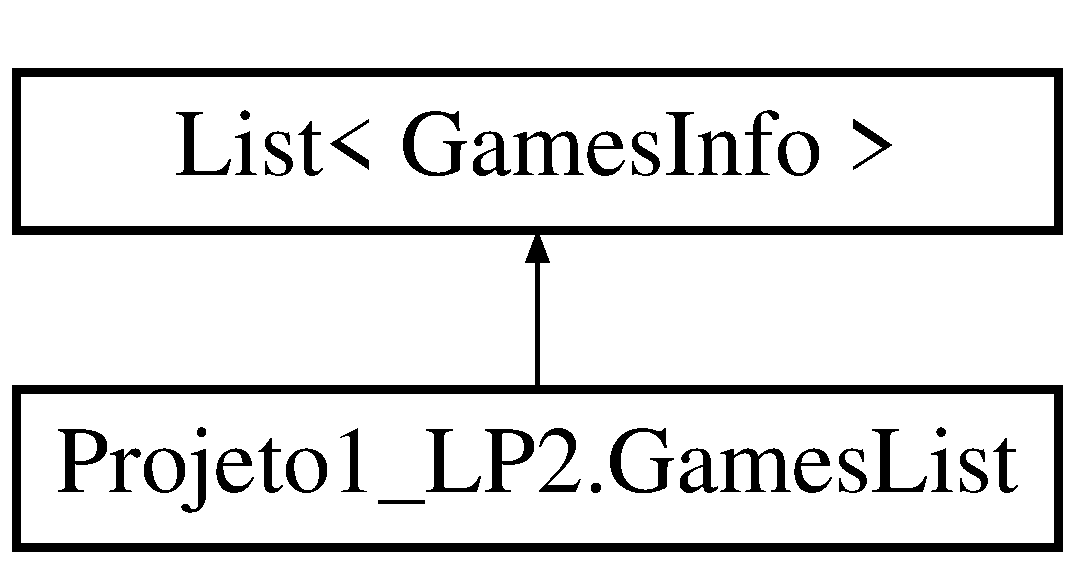
\includegraphics[height=2.000000cm]{class_projeto1___l_p2_1_1_games_list}
\end{center}
\end{figure}
\subsection*{Public Member Functions}
\begin{DoxyCompactItemize}
\item 
\hyperlink{class_projeto1___l_p2_1_1_games_list_a34bdf1752a0423357225757b3173f28f}{Games\+List} (string args)
\begin{DoxyCompactList}\small\item\em Constructor that will receive the argument from the command line \end{DoxyCompactList}\item 
void \hyperlink{class_projeto1___l_p2_1_1_games_list_abe89d421fc6fd99fdac598b82dbbc001}{Add\+Games} (string args)
\begin{DoxyCompactList}\small\item\em Method that will add the games from the comand line\textquotesingle{}s input \end{DoxyCompactList}\end{DoxyCompactItemize}


\subsection{Detailed Description}
Class that will inherit a list of \hyperlink{class_projeto1___l_p2_1_1_games_info}{Games\+Info} 



\subsection{Constructor \& Destructor Documentation}
\index{Projeto1\+\_\+\+L\+P2\+::\+Games\+List@{Projeto1\+\_\+\+L\+P2\+::\+Games\+List}!Games\+List@{Games\+List}}
\index{Games\+List@{Games\+List}!Projeto1\+\_\+\+L\+P2\+::\+Games\+List@{Projeto1\+\_\+\+L\+P2\+::\+Games\+List}}
\subsubsection[{\texorpdfstring{Games\+List(string args)}{GamesList(string args)}}]{\setlength{\rightskip}{0pt plus 5cm}Projeto1\+\_\+\+L\+P2.\+Games\+List.\+Games\+List (
\begin{DoxyParamCaption}
\item[{string}]{args}
\end{DoxyParamCaption}
)}\hypertarget{class_projeto1___l_p2_1_1_games_list_a34bdf1752a0423357225757b3173f28f}{}\label{class_projeto1___l_p2_1_1_games_list_a34bdf1752a0423357225757b3173f28f}


Constructor that will receive the argument from the command line 


\begin{DoxyParams}{Parameters}
{\em args} & \\
\hline
\end{DoxyParams}


\subsection{Member Function Documentation}
\index{Projeto1\+\_\+\+L\+P2\+::\+Games\+List@{Projeto1\+\_\+\+L\+P2\+::\+Games\+List}!Add\+Games@{Add\+Games}}
\index{Add\+Games@{Add\+Games}!Projeto1\+\_\+\+L\+P2\+::\+Games\+List@{Projeto1\+\_\+\+L\+P2\+::\+Games\+List}}
\subsubsection[{\texorpdfstring{Add\+Games(string args)}{AddGames(string args)}}]{\setlength{\rightskip}{0pt plus 5cm}void Projeto1\+\_\+\+L\+P2.\+Games\+List.\+Add\+Games (
\begin{DoxyParamCaption}
\item[{string}]{args}
\end{DoxyParamCaption}
)}\hypertarget{class_projeto1___l_p2_1_1_games_list_abe89d421fc6fd99fdac598b82dbbc001}{}\label{class_projeto1___l_p2_1_1_games_list_abe89d421fc6fd99fdac598b82dbbc001}


Method that will add the games from the comand line\textquotesingle{}s input 


\begin{DoxyParams}{Parameters}
{\em args} & \\
\hline
\end{DoxyParams}


The documentation for this class was generated from the following file\+:\begin{DoxyCompactItemize}
\item 
Projeto1\+\_\+\+L\+P2/\hyperlink{_games_list_8cs}{Games\+List.\+cs}\end{DoxyCompactItemize}

\hypertarget{class_projeto1___l_p2_1_1_interface_manager}{}\section{Projeto1\+\_\+\+L\+P2.\+Interface\+Manager Class Reference}
\label{class_projeto1___l_p2_1_1_interface_manager}\index{Projeto1\+\_\+\+L\+P2.\+Interface\+Manager@{Projeto1\+\_\+\+L\+P2.\+Interface\+Manager}}


Class that will manage what the user sees and inputs  


\subsection*{Public Member Functions}
\begin{DoxyCompactItemize}
\item 
\hyperlink{class_projeto1___l_p2_1_1_interface_manager_ab7e0f4ab529ccb9404b447780aca5b5c}{Interface\+Manager} (string args)
\begin{DoxyCompactList}\small\item\em The constructor of the class \end{DoxyCompactList}\item 
void \hyperlink{class_projeto1___l_p2_1_1_interface_manager_ae39278d41a699c7193d041daafd406af}{Show\+Menu} ()
\begin{DoxyCompactList}\small\item\em A method that will render the menu to the player \end{DoxyCompactList}\item 
int \hyperlink{class_projeto1___l_p2_1_1_interface_manager_a5f37f21c65d90767a37ff8ae13deed34}{Read\+Entry} ()
\begin{DoxyCompactList}\small\item\em Method that will read the player\textquotesingle{}s input and act accordingly \end{DoxyCompactList}\item 
void \hyperlink{class_projeto1___l_p2_1_1_interface_manager_a8b5597c81adbaca5791f7df826ead221}{Check\+ID} (int id)
\begin{DoxyCompactList}\small\item\em Method that will check the ID \end{DoxyCompactList}\end{DoxyCompactItemize}


\subsection{Detailed Description}
Class that will manage what the user sees and inputs 



\subsection{Constructor \& Destructor Documentation}
\index{Projeto1\+\_\+\+L\+P2\+::\+Interface\+Manager@{Projeto1\+\_\+\+L\+P2\+::\+Interface\+Manager}!Interface\+Manager@{Interface\+Manager}}
\index{Interface\+Manager@{Interface\+Manager}!Projeto1\+\_\+\+L\+P2\+::\+Interface\+Manager@{Projeto1\+\_\+\+L\+P2\+::\+Interface\+Manager}}
\subsubsection[{\texorpdfstring{Interface\+Manager(string args)}{InterfaceManager(string args)}}]{\setlength{\rightskip}{0pt plus 5cm}Projeto1\+\_\+\+L\+P2.\+Interface\+Manager.\+Interface\+Manager (
\begin{DoxyParamCaption}
\item[{string}]{args}
\end{DoxyParamCaption}
)}\hypertarget{class_projeto1___l_p2_1_1_interface_manager_ab7e0f4ab529ccb9404b447780aca5b5c}{}\label{class_projeto1___l_p2_1_1_interface_manager_ab7e0f4ab529ccb9404b447780aca5b5c}


The constructor of the class 


\begin{DoxyParams}{Parameters}
{\em args} & \\
\hline
\end{DoxyParams}


\subsection{Member Function Documentation}
\index{Projeto1\+\_\+\+L\+P2\+::\+Interface\+Manager@{Projeto1\+\_\+\+L\+P2\+::\+Interface\+Manager}!Check\+ID@{Check\+ID}}
\index{Check\+ID@{Check\+ID}!Projeto1\+\_\+\+L\+P2\+::\+Interface\+Manager@{Projeto1\+\_\+\+L\+P2\+::\+Interface\+Manager}}
\subsubsection[{\texorpdfstring{Check\+I\+D(int id)}{CheckID(int id)}}]{\setlength{\rightskip}{0pt plus 5cm}void Projeto1\+\_\+\+L\+P2.\+Interface\+Manager.\+Check\+ID (
\begin{DoxyParamCaption}
\item[{int}]{id}
\end{DoxyParamCaption}
)}\hypertarget{class_projeto1___l_p2_1_1_interface_manager_a8b5597c81adbaca5791f7df826ead221}{}\label{class_projeto1___l_p2_1_1_interface_manager_a8b5597c81adbaca5791f7df826ead221}


Method that will check the ID 


\begin{DoxyParams}{Parameters}
{\em id} & \\
\hline
\end{DoxyParams}
\index{Projeto1\+\_\+\+L\+P2\+::\+Interface\+Manager@{Projeto1\+\_\+\+L\+P2\+::\+Interface\+Manager}!Read\+Entry@{Read\+Entry}}
\index{Read\+Entry@{Read\+Entry}!Projeto1\+\_\+\+L\+P2\+::\+Interface\+Manager@{Projeto1\+\_\+\+L\+P2\+::\+Interface\+Manager}}
\subsubsection[{\texorpdfstring{Read\+Entry()}{ReadEntry()}}]{\setlength{\rightskip}{0pt plus 5cm}int Projeto1\+\_\+\+L\+P2.\+Interface\+Manager.\+Read\+Entry (
\begin{DoxyParamCaption}
{}
\end{DoxyParamCaption}
)}\hypertarget{class_projeto1___l_p2_1_1_interface_manager_a5f37f21c65d90767a37ff8ae13deed34}{}\label{class_projeto1___l_p2_1_1_interface_manager_a5f37f21c65d90767a37ff8ae13deed34}


Method that will read the player\textquotesingle{}s input and act accordingly 

\begin{DoxyReturn}{Returns}

\end{DoxyReturn}
\index{Projeto1\+\_\+\+L\+P2\+::\+Interface\+Manager@{Projeto1\+\_\+\+L\+P2\+::\+Interface\+Manager}!Show\+Menu@{Show\+Menu}}
\index{Show\+Menu@{Show\+Menu}!Projeto1\+\_\+\+L\+P2\+::\+Interface\+Manager@{Projeto1\+\_\+\+L\+P2\+::\+Interface\+Manager}}
\subsubsection[{\texorpdfstring{Show\+Menu()}{ShowMenu()}}]{\setlength{\rightskip}{0pt plus 5cm}void Projeto1\+\_\+\+L\+P2.\+Interface\+Manager.\+Show\+Menu (
\begin{DoxyParamCaption}
{}
\end{DoxyParamCaption}
)}\hypertarget{class_projeto1___l_p2_1_1_interface_manager_ae39278d41a699c7193d041daafd406af}{}\label{class_projeto1___l_p2_1_1_interface_manager_ae39278d41a699c7193d041daafd406af}


A method that will render the menu to the player 



The documentation for this class was generated from the following file\+:\begin{DoxyCompactItemize}
\item 
Projeto1\+\_\+\+L\+P2/\hyperlink{_interface_manager_8cs}{Interface\+Manager.\+cs}\end{DoxyCompactItemize}

\hypertarget{class_projeto1___l_p2_1_1_program}{}\section{Projeto1\+\_\+\+L\+P2.\+Program Class Reference}
\label{class_projeto1___l_p2_1_1_program}\index{Projeto1\+\_\+\+L\+P2.\+Program@{Projeto1\+\_\+\+L\+P2.\+Program}}


Class program  




\subsection{Detailed Description}
Class program 



The documentation for this class was generated from the following file\+:\begin{DoxyCompactItemize}
\item 
Projeto1\+\_\+\+L\+P2/\hyperlink{_program_8cs}{Program.\+cs}\end{DoxyCompactItemize}

\chapter{File Documentation}
\hypertarget{_games_info_8cs}{}\section{Projeto1\+\_\+\+L\+P2/\+Games\+Info.cs File Reference}
\label{_games_info_8cs}\index{Projeto1\+\_\+\+L\+P2/\+Games\+Info.\+cs@{Projeto1\+\_\+\+L\+P2/\+Games\+Info.\+cs}}
\subsection*{Classes}
\begin{DoxyCompactItemize}
\item 
class \hyperlink{class_projeto1___l_p2_1_1_games_info}{Projeto1\+\_\+\+L\+P2.\+Games\+Info}
\begin{DoxyCompactList}\small\item\em Class that will store all the needed variables \end{DoxyCompactList}\end{DoxyCompactItemize}
\subsection*{Namespaces}
\begin{DoxyCompactItemize}
\item 
namespace \hyperlink{namespace_projeto1___l_p2}{Projeto1\+\_\+\+L\+P2}
\end{DoxyCompactItemize}

\hypertarget{_games_list_8cs}{}\section{Projeto1\+\_\+\+L\+P2/\+Games\+List.cs File Reference}
\label{_games_list_8cs}\index{Projeto1\+\_\+\+L\+P2/\+Games\+List.\+cs@{Projeto1\+\_\+\+L\+P2/\+Games\+List.\+cs}}
\subsection*{Classes}
\begin{DoxyCompactItemize}
\item 
class \hyperlink{class_projeto1___l_p2_1_1_games_list}{Projeto1\+\_\+\+L\+P2.\+Games\+List}
\begin{DoxyCompactList}\small\item\em Class that will inherit a list of \hyperlink{class_projeto1___l_p2_1_1_games_info}{Games\+Info} \end{DoxyCompactList}\end{DoxyCompactItemize}
\subsection*{Namespaces}
\begin{DoxyCompactItemize}
\item 
namespace \hyperlink{namespace_projeto1___l_p2}{Projeto1\+\_\+\+L\+P2}
\end{DoxyCompactItemize}

\hypertarget{_interface_manager_8cs}{}\section{Projeto1\+\_\+\+L\+P2/\+Interface\+Manager.cs File Reference}
\label{_interface_manager_8cs}\index{Projeto1\+\_\+\+L\+P2/\+Interface\+Manager.\+cs@{Projeto1\+\_\+\+L\+P2/\+Interface\+Manager.\+cs}}
\subsection*{Classes}
\begin{DoxyCompactItemize}
\item 
class \hyperlink{class_projeto1___l_p2_1_1_interface_manager}{Projeto1\+\_\+\+L\+P2.\+Interface\+Manager}
\begin{DoxyCompactList}\small\item\em Class that will manage what the user sees and inputs \end{DoxyCompactList}\end{DoxyCompactItemize}
\subsection*{Namespaces}
\begin{DoxyCompactItemize}
\item 
namespace \hyperlink{namespace_projeto1___l_p2}{Projeto1\+\_\+\+L\+P2}
\end{DoxyCompactItemize}

\hypertarget{_program_8cs}{}\section{Projeto1\+\_\+\+L\+P2/\+Program.cs File Reference}
\label{_program_8cs}\index{Projeto1\+\_\+\+L\+P2/\+Program.\+cs@{Projeto1\+\_\+\+L\+P2/\+Program.\+cs}}
\subsection*{Classes}
\begin{DoxyCompactItemize}
\item 
class \hyperlink{class_projeto1___l_p2_1_1_program}{Projeto1\+\_\+\+L\+P2.\+Program}
\begin{DoxyCompactList}\small\item\em Class program \end{DoxyCompactList}\end{DoxyCompactItemize}
\subsection*{Namespaces}
\begin{DoxyCompactItemize}
\item 
namespace \hyperlink{namespace_projeto1___l_p2}{Projeto1\+\_\+\+L\+P2}
\end{DoxyCompactItemize}

%--- End generated contents ---

% Index
\backmatter
\newpage
\phantomsection
\clearemptydoublepage
\addcontentsline{toc}{chapter}{Index}
\printindex

\end{document}
